\setcounter{chapter}{-1}
\chapter{绪论}

本节旨在作为文化导入，逻辑上不属于课程内容，可略读.

\section{内容简介}

代数簇(variety)大致可以定义为由多项式方程族定义的轨迹:

\[
V = \left\{  {P \in  {k}^{n} \mid  {f}_{i}\left( P\right)  = 0}\right\}   \subset  {k}^{n},
\]

其中 \(k\) 是一个域， \({f}_{i} \in  k\left\lbrack  {{X}_{1},\ldots ,{X}_{n}}\right\rbrack\) 是多项式；例如，平面曲线 \(C\) : \(\left( {f\left( {x,y}\right)  = 0}\right)  \subset  {\mathbb{R}}^{2}\) 或 \({\mathbb{C}}^{2}\) .

\begin{center}
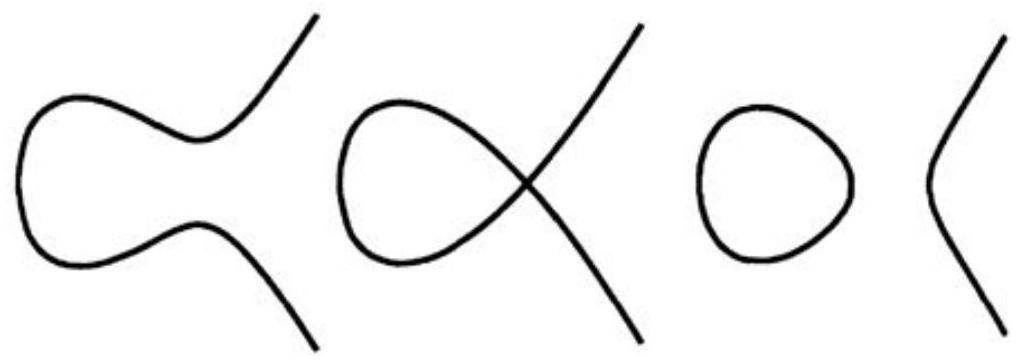
\includegraphics[max width=0.8\textwidth]{images/bo_d3lj80c601uc738kffi0_8_333_1201_1024_361_0.jpg}
\captionof{figure}{三次曲线 (a) \({y}^{2} = \left( {x + 1}\right) \left( {{x}^{2} + \varepsilon }\right) ,\;\) (b) \({y}^{2} = \left( {x + 1}\right) {x}^{2}\)，(c) \({y}^{2} = \left( {x + 1}\right) \left( {{x}^{2} - \varepsilon }\right)\)}.
\end{center}


如果我想研究 \(V\)，自然会产生以下几个问题:

\textbf{数论问题}\quad 例如，如果 \(k = \mathbb{Q}\) 和 \(V \subset  {\mathbb{Q}}^{n}\) ，如何判断 \(V\) 是否非空，若非空如何找到所有点？一个具体案例在历史上颇具意义：下列方程解的个数问题
\[
{x}^{n} + {y}^{n} = 1\text{ ,其中}x,y \in  \mathbb{Q}\text{且}n \geq  3\text{ ? }
\]

此类问题通常称为丢番图问题(Diophantine problems).

\textbf{拓扑问题}\quad 如果 \(k\) 是 \(\mathbb{R}\) 或 \(\mathbb{C}\) (常见情形)，那么 \(V\) 是什么样的拓扑空间？例如，上述三次曲线的连通分支就是明显的拓扑不变量.

\textbf{奇异性问题}\quad \(V\) 在 \(P \in  V\) 附近是什么样的拓扑空间；如果 \(f : {V}_{1} \rightarrow  {V}_{2}\) 是两个簇之间的正则映射(例如，多项式映射 \({\mathbb{R}}^{2} \rightarrow  \mathbb{R}\) )，那么 \(f\) 在 \(P \in  {V}_{1}\) 附近具有怎样的拓扑和几何结构？

\section{具体计算与一般理论}

研究簇有两种可能的方法:

具体的 给定特定的多项式 \({f}_{i}\) ，我们常常可以通过对 \({f}_{i}\) 的显式技巧来理解簇 \(V\) ；当维数 \(n\) 和 \({f}_{i}\) 的次数较小时，或者 \({f}_{i}\) 特别简单时，这很有趣，但情况会逐渐复杂，很快就会出现仅凭计算的巧思无法揭示问题本质的时刻.

一般的 对 \(V\) 性质的研究立即引出基本概念，如 \(V\) 上的正则函数(regular functions)、非奇异性(nonsingularity)和切平面、簇的维数:曲线如上述三次曲线是一维的这一观念在初等笛卡尔几何中很熟悉，图像也立即暗示了奇异点的含义.

现在，开设本科代数几何课程的一个基本问题是，对“通用”方法的充分讲解涉及大量定义，这些定义占满整个课程，挤压了实质内容.因此必须妥协，我的解决方案是覆盖一般理论的一小部分，并不断参照具体例子.因此这些讲义仅包含构成三年本科数学课程中专门代数几何必修核心的“标准教材”内容的一小部分.另一方面，我希望每节都包含一些有实质内容的习题和例题.

\section{函数环与几何范畴}

代数几何的特殊风格源于仅使用多项式函数(以及有理函数)；为说明这一点，若 \(U \subset  {\mathbb{R}}^{2}\) 是一个开区间，则可以合理地考虑以下定义在 \(U\) 上的函数环:

\begin{itemize}
\item \({C}^{0}\left( U\right)  =\) 所有连续函数 \(f : U \rightarrow  \mathbb{R}\) ；
\end{itemize}

\begin{itemize}
\item \({C}^{\infty }\left( U\right)  =\) 所有光滑函数(即任意阶可微)；
\end{itemize}

\begin{itemize}
\item \({C}^{\omega }\left( U\right)  =\) 所有解析函数(即收敛幂级数)；
\end{itemize}

\begin{itemize}
\item \(\mathbb{R}\left\lbrack  X\right\rbrack   =\) 多项式环，视为定义在 \(U\) 上的多项式函数.
\end{itemize}

当然存在包含关系 \(\mathbb{R}\left\lbrack  X\right\rbrack   \subset  {C}^{\omega }\left( U\right)  \subset  {C}^{\infty }\left( U\right)  \subset  {C}^{0}\left( U\right)\) .

这些函数环对应于几何学中的一些重要范畴: \({C}^{0}\left( U\right)\) 对应拓扑范畴， \({C}^{\infty }\left( U\right)\) 对应可微范畴(可微流形)， \({C}^{\omega }\) 对应实解析几何， \(\mathbb{R}\left\lbrack  X\right\rbrack\) 对应代数几何.我想强调的是，每一个包含符号都代表着一个极其巨大的鸿沟，这导致了不同范畴中几何的主要特征.虽然在学校和大学一年级的微积分中并未强调，但任何合理的测度方式 \({C}^{0}\left( U\right)\) 都会显示可微函数在连续函数中测度为零(因此如果随机选取一个连续函数，几乎必然处处不可微，如布朗运动). \({C}^{\omega }\left( U\right)\) 与 \({C}^{\infty }\left( U\right)\) 之间的差距通过标准函数 \(\exp \left( {-1/{x}^{2}}\right)\) 的行为得以体现，该函数可微无数次，但其在0点的泰勒级数不收敛于 \(f\) ；利用此函数，可以轻松构造一个 \({C}^{\infty }\) “凸起函数” \(f : \mathbb{R} \rightarrow  \mathbb{R}\) ，使得当 \(\left| x\right|  \leq  {0.9}\) 时 \(f\left( x\right)  = 1\) ，当 \(\left| x\right|  \geq  1\) 时 \(f\left( x\right)  = 0\) .相比之下，定义在 \(U\) 上的解析函数可作为复变量的解析函数(幂级数收敛)延拓到 \({C}^{0}\left( U\right)\) 中合适的区域，因此(利用复分析的结果)，如果 \({C}^{\infty }\left( U\right)\) 在实区间上恒为零，则必在整体上恒为零.这是一种“刚性”性质，区别了解析几何与微分拓扑.

\begin{center}
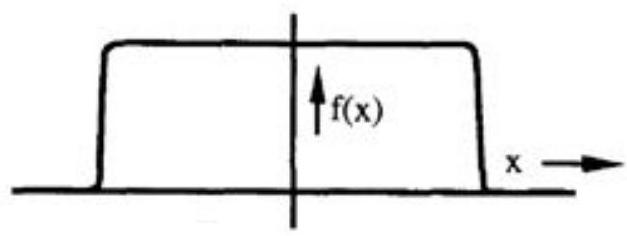
\includegraphics[max width=0.4\textwidth]{images/bo_d3lj80c601uc738kffi0_10_531_651_627_236_0.jpg}
\end{center}
\hspace*{3em} 

图2:一个 \({C}^{\infty }\) 凸起函数.

幂级数)延拓为复变量的解析函数，定义在 \(\mathbb{C}\) 中合适的区域，因此(利用复分析的结果)，如果 \(f \in  {C}^{\omega }\left( U\right)\) 在实区间上恒为零，则必在整体上恒为零.这是一种“刚性”性质，区别了解析几何与微分拓扑.

\section{多项式几何}

多项式函数非常稀少:多项式环 \(\mathbb{R}\left\lbrack  X\right\rbrack\) 只是一个可数维的 \(\mathbb{R}\) -向量空间，而 \({C}^{\omega }\left( U\right)\) 已经是不可数的.即使允许有理函数——即将 \(\mathbb{R}\left\lbrack  X\right\rbrack\) 扩展到其分式域 \(\mathbb{R}\left( X\right)\) ——也帮助不大.(2.2)将提供代数范畴特有刚性的一个例子.仅用这组函数构建几何本身就相当了不起.不出所料，建立这一理论存在诸多困难:

通过交换代数的基础 拓扑学和微分拓扑学可以依赖于一系列 \(\varepsilon  - \delta\) 分析课程中教授的全部内容，这些课程通常为 \(1\mathrm{{st}}\) 和 \(2\mathrm{{nd}}\) 年制的本科课程；而要仅用多项式环来进行代数几何研究，我们则需要研究诸如多项式环 \(k\left\lbrack  {{X}_{1},\ldots ,{X}_{n}}\right\rbrack\) 及其理想等环.换句话说，我们必须发展交换代数以替代微积分.Nullstellensatz(下文的 \(§3\) )是一个典型例子，它是一个具有直接直观几何内容的命题(本质上是“多项式环 \(k\left\lbrack  {{X}_{1},\ldots ,{X}_{n}}\right\rbrack\) 中不同的函数理想定义不同的簇(varieties) \(V \subset  {k}^{n}\) ”)，其证明涉及交换代数中有限性条件的较长论述.

有理映射和函数 由于选择仅用多项式进行研究，另一个难点是必须引入“部分定义的函数”；正如上文所暗示的“刚性”，我们将看到对于某些簇(实际上是所有射影簇)，不存在任何非恒定的正则函数(参见例5.1、例5.12及(8.10)中的讨论).有理函数(即形如 \(f = g/h\) 的“函数”，其中 \(g,h\) 是多项式函数)在分母为零的点处未定义.尽管令人诟病，但代数几何学家中有一种根深蒂固的传统，将“有理函数”和“有理映射”理解为“仅部分定义的函数(或映射)”.因此，有理映射 \(f : {V}_{1} \rightarrow  {V}_{2}\) 实际上根本不是映射；这里的断箭头也逐渐成为惯例.不赞同者建议立即放弃，转而选修范畴论的阅读课程.

这绝非轻率的问题.即使是正则映射(即态射，是真正的映射)也必须定义为在所有点 \(P \in  V\) 处正则的有理映射(即定义良好，分母可选取为在 \(P\) 处不为零).与此密切相关的是给出簇的恰当内在定义的难题:在本课程(以及我所知的类似课程)中，将定义仿射簇 \(V \subset  {\mathbb{A}}^{n}\) 和拟射影簇 \(V \subset  {\mathbb{P}}^{n}\) ，但不会给出不依赖于环境空间的“簇”的恰当定义.粗略地说，簇应当是将若干仿射簇沿同构的开子集粘合而成的对象.但我们目前的语言中，同构本身多半是通过有理函数明确定义的，过于繁琐；而这种粘合的恰当语言是层(sheaves)，这在研究生教材中有较好论述.

\section{“纯代数定义”}

以上即代数几何方法的缺点.话虽如此，现今世界上几乎所有重要的代数簇都是拟射影簇，我们可以在不太纠结定义细节的情况下，尽情享受簇的乐趣.

代数几何的主要优势在于它是纯代数定义的，且适用于任意域，而不仅仅是 \(\mathbb{R}\) 或 \(\mathbb{C}\) ；我们可以在特征为 \(p\) 的域上做几何.不要说“特征为 \(p\) ——没什么大不了的，那只是有限域”；首先，群论中相当重要的部分基于有限域上的几何，计算机科学中使用的组合学的很大一部分也是如此.其次，存在许多有趣的非有限的特征为 \(p\) 的域.此外，在深层次上，有限域存在并作用于 \(\mathbb{Q}\) 和 \(\mathbb{C}\) 中.关于在 \(\mathbb{Q}\) 上的簇的算术的许多深刻结果，都大量使用了在 \(\mathbb{C}\) 或有限域及其代数闭包上的几何.

介绍到此结束；更多通识内容请参见(2.15)中的非正式讨论及最后的 \(§8\) .

\section{本书计划}

关于本书的结构，第一部分和第三部分旨在指出一些可以通过代数几何方法研究的有价值的问题.第二部分是对(0.4)中提到的交换代数及代数几何的范畴框架的介绍；容易头疼的学生或许可以将其中一些证明视为理所当然，因为这些内容是标准的，且作者是一位具有最高道德品质的专业代数几何学家.

\(§8\) 包含一些可能对学生有兴趣或有用但不适合放入正文的零碎内容:现代学科的一些历史和社会学，关于该学科与更高级主题关系的提示，技术性脚注等.

\section{本课程的先修知识:}

代数:二次型，交换环及其理想的基本性质，主理想整环和唯一分解.

伽罗瓦理论:域，多项式环，有限扩张，代数扩张与超越扩张，分离性.

拓扑与几何:拓扑空间的定义，射影空间 \({\mathbb{P}}^{n}\) (但我会再次详细讲解).

\({\mathbb{R}}^{n}\) 中的微积分:偏导数，隐函数定理(但当我们讲到时我会提醒你所需内容).

交换代数:有其他交换环的经验是可取的，但不是必需的.

\section{课程相关领域:}

复变函数论:定义在 \(\mathbb{C}\) 上的代数曲线是一维复流形，其上的正则函数是全纯函数，因此本课程与复变函数论密切相关，尽管这种关系不一定立刻显现.

代数数论:例如与费马大定理的关系.

灾变理论:灾变是奇点，且本质上总是由多项式函数给出，因此奇点几何的分析是纯粹的代数几何.

交换代数:代数几何为交换代数提供动机，交换代数为代数几何提供技术支持，两者相辅相成.

\section{第0章习题}

0.1 (a) 证明对于固定的值， \(\left( {y,z}\right) ,x\) 是 \({x}^{3} + {xy} + z = 0\) 的重根当且仅当 \(x =  - {3z}/{2y}\) 和 \(4{y}^{3} + {27}{z}^{2} = 0\) ；

(b) 当且仅当 \(4{y}^{3} + {27}{z}^{2} < 0\) 时有3个不同的根；

(c) 画出曲面 \(S : \left( {{x}^{3} + {xy} + z = 0}\right)  \subset  {\mathbb{R}}^{3}\) 及其在(y, z)平面上的投影；

(d) 现在翻开任何一本关于灾变理论的书籍或文章进行比较.

0.2 设 \(f \in  \mathbb{R}\left\lbrack  {X,Y}\right\rbrack\) 且设 \(C : \left( {f = 0}\right)  \subset  {\mathbb{R}}^{2}\) ；若存在 \(\varepsilon  > 0\) 使得 \(C \cap  B\left( {P,\varepsilon }\right)  = P\) ，则称 \(P \in  C\) 为孤立点.举例说明 \(C\) 可以有孤立点.证明若 \(P \in  C\) 是孤立点，则 \(f : {\mathbb{R}}^{2} \rightarrow  \mathbb{R}\) 在 \(P\) 处必有极大值或极小值，并推导出 \(\frac{\partial f}{\partial x}\) 和 \(\frac{\partial f}{\partial y}\) 在 \(P\) 处消失.这证明了实曲线的孤立点是奇异点.

0.3 三次曲线:

(i) 画出 \(y = 4{x}^{3} + 6{x}^{2}\) 的图形及其与水平线 \(y = t\) ( \(t \in  \left\lbrack  {-1,3}\right\rbrack\) 取整数值)交点；

(ii) 画出相同 \(t\) 值下的三次曲线 \({y}^{2} = 4{x}^{3} + 6{x}^{2} - t\) .

\section*{书籍}

以下大多数为研究生水平的教材，部分在正文中有引用:

W. Fulton，《代数曲线》(Algebraic curves)，Springer.(这是研究生教材中最通俗且自成体系的；第1-6章非常适合本科课程，尽管内容略显枯燥.)

I.R. Shafarevich，《基础代数几何》(Basic algebraic geometry)，Springer.(研究生教材，但第I章和SII.1节内容相当适合.)

P. Griffiths 和 J. Harris，《代数几何原理》(Principles of algebraic geometry)，Wiley.(提供复分析视角.)

David Mumford，《代数几何I:复射影簇》(Algebraic geometry I, Complex projective varieties)，Springer.

D. Mumford，《代数几何导论》(Introduction to algebraic geometry)，哈佛讲义.(起初不易读，但直指要点；我这一代许多代数几何学家都是从这套讲义学艺的.最近作为Springer LNM 1358重新出版，因此不再是那本小红书.)

K. Kendig，《初等代数几何》(Elementary algebraic geometry)，Springer.(论述代数几何与复分析几何的关系.)

R. Hartshorne，《代数几何》(Algebraic geometry)，Springer.(这是专业人士的手册，涵盖更高级内容；第I章为本科课程的简要纲要.)

M. Berger，《几何学I和II》(Geometry I and II)，Springer.(第二册中关于二次型和二次超曲面的章节内容尤为相关.)

M.F. Atiyah 和 I.G. Macdonald，《交换代数》，Addison-Wesley.(一本极其宝贵的教材.)

E. Kunz，《交换代数与代数几何导论》，Birkhäuser.

H. Matsumura，《交换环论》，Cambridge.(一本关于交换代数更为详尽的著作.)

D. Mumford，《曲线及其雅可比簇》，密歇根大学出版社.(通俗讲座，讲得既深入又迅速.)

C.H. Clemens，《复曲线剪贴簿》，Plenum.(非常有趣.)

E. Brieskorn 和 H. Knörrer，《平面代数曲线》，Birkhäuser.

A. Beauville，《复代数曲面》，LMS讲义，Cambridge.

J. Kollár，《代数三重体的结构:Mori计划导论》，美国数学学会公报 17 (1987), 211-273.(一份对一个活跃研究领域的精美介绍手册.基本无害.)

J.G. Semple 和 L. Roth，《代数几何导论》，Oxford.(一本精彩的老书，信息丰富，但几乎完全缺乏严谨性.)

J.L. Coolidge，《代数平面曲线论》，Oxford 和 Dover.